\documentclass[11pt]{article}

\usepackage{amsmath}
\usepackage{amssymb}
\usepackage{textcomp}
\usepackage{graphicx}
\graphicspath{ {./} }
\usepackage{wrapfig}
\usepackage[top=0.8in, bottom=0.8in, left=0.8in, right=0.8in]{geometry}
% Add other packages here %


% Put your group number and names in the author field %
\title{\bf Excercise 4\\ Implementing a centralized agent}
\author{Group \textnumero : 90  Kyle Gerard, Yann Bolliger}


% N.B.: The report should not be longer than 3 pages %


\begin{document}
 \maketitle

 \section{Solution Representation}

 \subsection{Variables}

 Instead of representing a vehicle's journey as a sequence of tasks, we chose to
 represent it as a sequence of $pickup$ and $delivery$ actions. Each task $t \in
 \mathcal{T}$ has one action of both types (\ref{eq:1}). This accounts for the
 fact that a vehicle can carry multiple tasks at a time if there are two pickups
 in a row.
 The variables (\ref{eq:2}) define the first pickup of each vehicle
 $v \in \mathcal{V}$. If the variable is $\mathtt{null}$ this means the vehicle
 does not accomplish any actions.
 \begin{eqnarray}
  \label{eq:1}
  \mathcal{P} = \{pickup(t) : t \in \mathcal{T}\} , \;
  \mathcal{D} = \{delivery(t) : t \in \mathcal{T}\} , \;
  \mathcal{A} =  \mathcal{P} \cup \mathcal{D}
  \\
  \label{eq:2}
  \forall v \in \mathcal{V}  : \;
  firstPickup(v)  \in \mathcal{P} \cup \{\mathtt{null}\}
  \\
  \label{eq:3}
  \forall a \in \mathcal{A}  : \;
  nextAction(a) \in \mathcal{A}  \cup \{\mathtt{null}\}
  \\
  \label{eq:4}
  \forall a \in \mathcal{A}  :
  vehicle(a) \in \mathcal{V};
  \;\;
  \forall a \in \mathcal{A}  :
  time(a) \in \mathbb{N}
 \end{eqnarray}

 A vehicles journey is completely defined by its $firstPickup$ and the variables
 (\ref{eq:3}) where again the $\mathtt{null}$ signifies that a vehicle has no
 further actions to perform. We will call the sequence of actions of a vehicle
 its action chain. All travels are made on the shortest possible path.

 The variables (\ref{eq:4}) help us state the constraints. The $vehicle$
 variables define which vehicle carries out a certain action. This can be derived
 from $firstPickup$ at the start of the action chain defined by (\ref{eq:3}). The
 second variable can also be derived from the action chains. It simply gives the
 rank of each action in the chain. Both derivations are more formally stated in
 the next paragraph.

 \subsection{Constraints}
 As explained before, the action chain of a vehicle defines the $time$
 and the $vehicle$ for each action:
 \begin{eqnarray}
  firstPickup(v) = a \Rightarrow vehicle(a) = v;  &
  nextAction(b)  = c \Rightarrow vehicle(c) = vehicle(b)
  \\
  firstPickup(v) = a \Rightarrow time(a) = 1;  &
  nextAction(b)  = c \Rightarrow time(c) = time(b) + 1
 \end{eqnarray}

 Additionally, the same vehicle must $pickup$ and $deliver$ a task (\ref{eq:v}).
 It has to pickup the task before it delivers it (\ref{eq:t})
 and \textbf{each task must be picked up and delivered}.
 \begin{eqnarray}
  \forall a \in \mathcal{A}  :
  nextAction(a) \neq a
  \\
  nextAction(a) = \mathtt{null} \Rightarrow a \in \mathcal{D}
  \text{ and } nextAction(\mathtt{null}) = \mathtt{null}
  \\
  \label{eq:v}
  \forall t \in \mathcal{T}:
  vehicle(pickup(t)) = vehicle(delivery(t))
  \\
  \label{eq:t}
  \forall t \in \mathcal{T}:
  time(pickup(t)) < time(delivery(t))
  \\
  \forall t \in \mathcal{T} \;
  \exists  \, \{ pickup(t), delivery(t) \} \subset \mathcal{A} \;\;
  \\
  \forall a \in \mathcal{A} \;
  \exists \, v \in \mathcal{V} :
  vehicle(a) = v
 \end{eqnarray}

 Last but not least, at all times $\tau$ a vehicle $v$ can never
 carry more weight than its capacity.
 $$
 carriedTasks(\tau, v) = \{t \in \mathcal{T}:
 vehicle(pickup(t)) = v \wedge
 time(pickup(t)) < \tau \wedge
 time(delivery(t)) > \tau \}
 $$$$
 \forall \tau \in \mathbb{N},
 \forall v \in \mathcal{V}:
 \sum_{t \, \in \, carriedTasks(\tau, v)} weight(t) \leq
 capacity(v)
 $$

 \subsection{Objective function}

 The goal of the company is to maximise the reward. Because all tasks have to be
 delivered, all rewards will be earned and the overall reward is constant. Thus
 the objective function we want to minimise is the cost of the overall assignment
 $\mathcal{S}$. We define $dist(a,b)$ to be the shortest distance between the
 associated cities of actions $a,b \in \mathcal{A}$, $dist(a, \mathtt{null}) =
 0$, $start(v)$ is the initial postion and $cost(v)$ the cost per kilometre of
 vehicle $v$.
 $$
 cost(\mathcal{S}) =
 \sum_{v \in \mathcal{V}} dist(start(v), firstPickup(v))
 \cdot cost(v)
 +
 \sum_{a \in \mathcal{A}} dist(a, nextAction(a))
 \cdot cost(vehicle(a))
 $$


 \section{Stochastic optimization}

 \subsection{Initial solution}

 Our initial solution is already a valid, greedy solution. Therefore, our program
 returns a correct assignment at all times, even if there is no computation time.
 The initial solution is computed by appending consecutively the $pickup$ and
 $delivery$ pair of each task to the action chain of the vehicle that is the
 closest (and has enough capacity). This distance is calculated between the last
 position in the action chain of each vehicle and the $pickup$ location.
 Therefore in the initial solution the vehicles don't carry multiple tasks at
 once.


 \subsection{Generating neighbours}

 We generate neighbors of a current assignment $\mathcal{S}$ by applying two
 stochastic operators. For both of them, we randomly choose a vehicle $v$. Then,
 for the first set of neighbors, we remove both actions $p, d$ for a random task
 $t$ from the action chain of $v$. The neighbors result from inserting $p, d$
 into the action chains of all other neighbors. This yields a lot of
 possibilities because the $p, d$ can be inserted in many ways into the new
 action chain as long as the capacity and the $p$ before $d$ constraint is
 respected. The second set of neighbors is obtained from reordering the actions
 in $v$'s chain without removing or inserting. Still the reordering has to
 respect the capacity and the $p$ before $d$ constraint.


 \subsection{Stochastic optimization algorithm}

 As proposed in the paper\footnote{Radu Jurca, Nguyen Quang Huy and Michael
 Schumacher {\em Finding the Optimal Delivery Plan: Model as a Constraint
 Satisfaction Problem} 2006-2007: Intelligent Agents course} we use stochastic
 local search to find a better solution than the initial one. Thereby we generate
 neighbors at each iteration and with probability $p$, we take the least costly
 neighbor as a new solution.

 We made a critical addition to the algorithm that avoids getting stuck in local
 minima. In fact, if there are two pickups at the same location, this yields two
 solutions depending on the order of the pickups. However, the solutions are
 completely equivalent in terms of cost. Therfore, each time a new solution is
 chosen, we add this solution to a set called \texttt{formerSolutions}. In
 addition, the algorithm is not allowed to subsequently choose a solution with
 the \textbf{same cost} as one that is already in the set. In that manner it has
 to keep exploring new solutions with new and possibly lower cost. At the end
 the overall minimum that was ever visited is returned.


 \section{Results}

 \subsection{Experiment 1: Model parameters}
 % if your model has parameters, perform an experiment and
 % analyze the results for different parameter values %

 \subsubsection{Setting}
 % Describe the settings of your experiment: topology,
 % task configuration, number of tasks, number of vehicles, etc. %
 % and the parameters you are analyzing %
 Default configuration given in handout (30 tasks, 4 cars). Probability $p$
 between 0 and 0.9 
 
 \subsubsection{Observations} 
 % Describe the experimental results and the
 % conclusions you inferred from these results %
 
 \begin{wrapfigure}{R}{0.55\textwidth}
    \vspace{-20pt}
 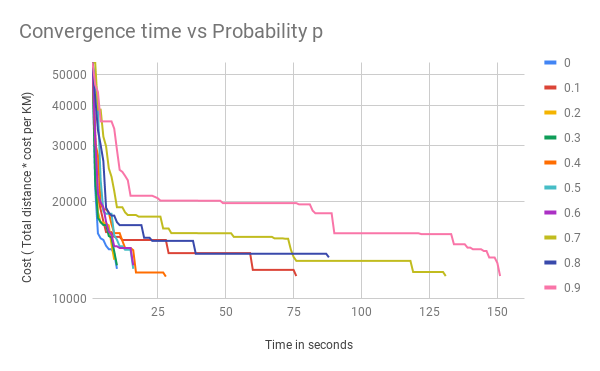
\includegraphics[width=0.55\textwidth]{convergence.png} 
   \vspace{-20pt}
 \end{wrapfigure} 
 
 As we can see in the graph on the right, a higher probability $p$ value takes
 more time to converge towards an optimal solution than lower $p$ values. This
 makes sense because with a high probability $p$ it is likely that the algorithm
 choose a new solution more often. Thus more solutions are generated. 
 
 Other than the time to converge to a good solution, the cost of the final
 solution itself (given enough time) does not seem to depend on the probability
 $p$. Indeed, after 3 minutes, all plans cost between 10,000 and 13,000 which is
 a relatively small range.



 \subsection{Experiment 2: Different configurations}
 % Run simulations for different configurations of the environment
 % (i.e. different tasks and number of vehicles) %

 \subsubsection{Setting}
 % Describe the settings of your experiment: topology, task
 % configuration, number of tasks, number of vehicles, etc. %
 Default configuration with tasks from 1 to 40 and number of cars from 1 to 4.

 \subsubsection{Observations}
 % Describe the experimental results and the conclusions you inferred
 % from these results. Reflect on the fairness of the optimal plans.
 % Observe that optimality requires some vehicles to do more work
 % than others. How does the complexity of your algorithm depend on the
 % number of vehicles and various sizes of the task set? %
 
 Changing the number of cars has very little influence on the cost of a plan.
 Indeed, with one car (and 30 tasks) we were able to find a plan with a cost of
 12'451 and with four cars we found a plan with a cost of 11'703. The reason for
 this small difference in cost is that in the better solution with four cars
 only one car is actually delivering tasks. This is because there is no notion
 of time efficiency to deliver all tasks, only the distance travelled is
 relevant. It is therefore normal that you can obtain similar results using only
 one car and that plans with multiple cars are unfair (some drivers will not
 deliver any tasks).
\\

 \begin{wrapfigure}{L}{0.5\textwidth}
  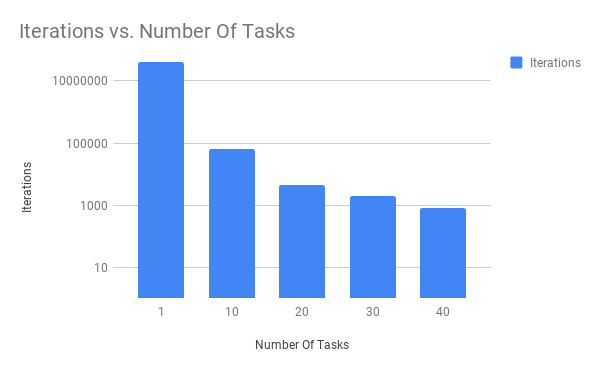
\includegraphics[width=0.5\textwidth]{iterations.png}
   \vspace{-20pt}
 \end{wrapfigure}
 
 
 In the graph on the left we see that the complexity of the algorithm increases
 with the number of tasks. This is to be expected as in every iteration of the
 algorithm we calculate the possible neighbors as explained in part 2.2. Finding
 all possible combinations of pickups and deliveries of a plan takes time
 $\mathcal{O}(n^3)$, where $n$ is the number of tasks in the plan. 
 
 The complexity of our algorithm is however not dependent on the number of
 vehicles because tasks are not evenly distributed between cars (most cars take
 constant time $\mathcal{O}(n^3) = \mathcal{O}(1)$ per iteration as no tasks are
 given to them $n=0$).

\end{document}